\chapter{Data generation and storage}
\label{chap:data}

\section{Introduction}
\label{sec:intro_data}

This chapter gathers several proposals related with the creation, storage and transmission of ambisonic data for research purposes. The main objective of the contributions described here is the support for the generation of parametrizable ambisonic datasets, using both synthetic and recorded materials, and specifically emphasizing the usage of Room Impulse Responses.\\ 

Most of the contributions listed here (and also most of the code developed for this thesis) have been implemented in Python. Indeed, Python has recently become one of the most used programming languages worldwide \cite{theoverflow, PYPL, TIOBE}; as shown also in Figure~\ref{fig:popularity}.\\

\begin{figure}
\label{fig_architecture}
  \centering
    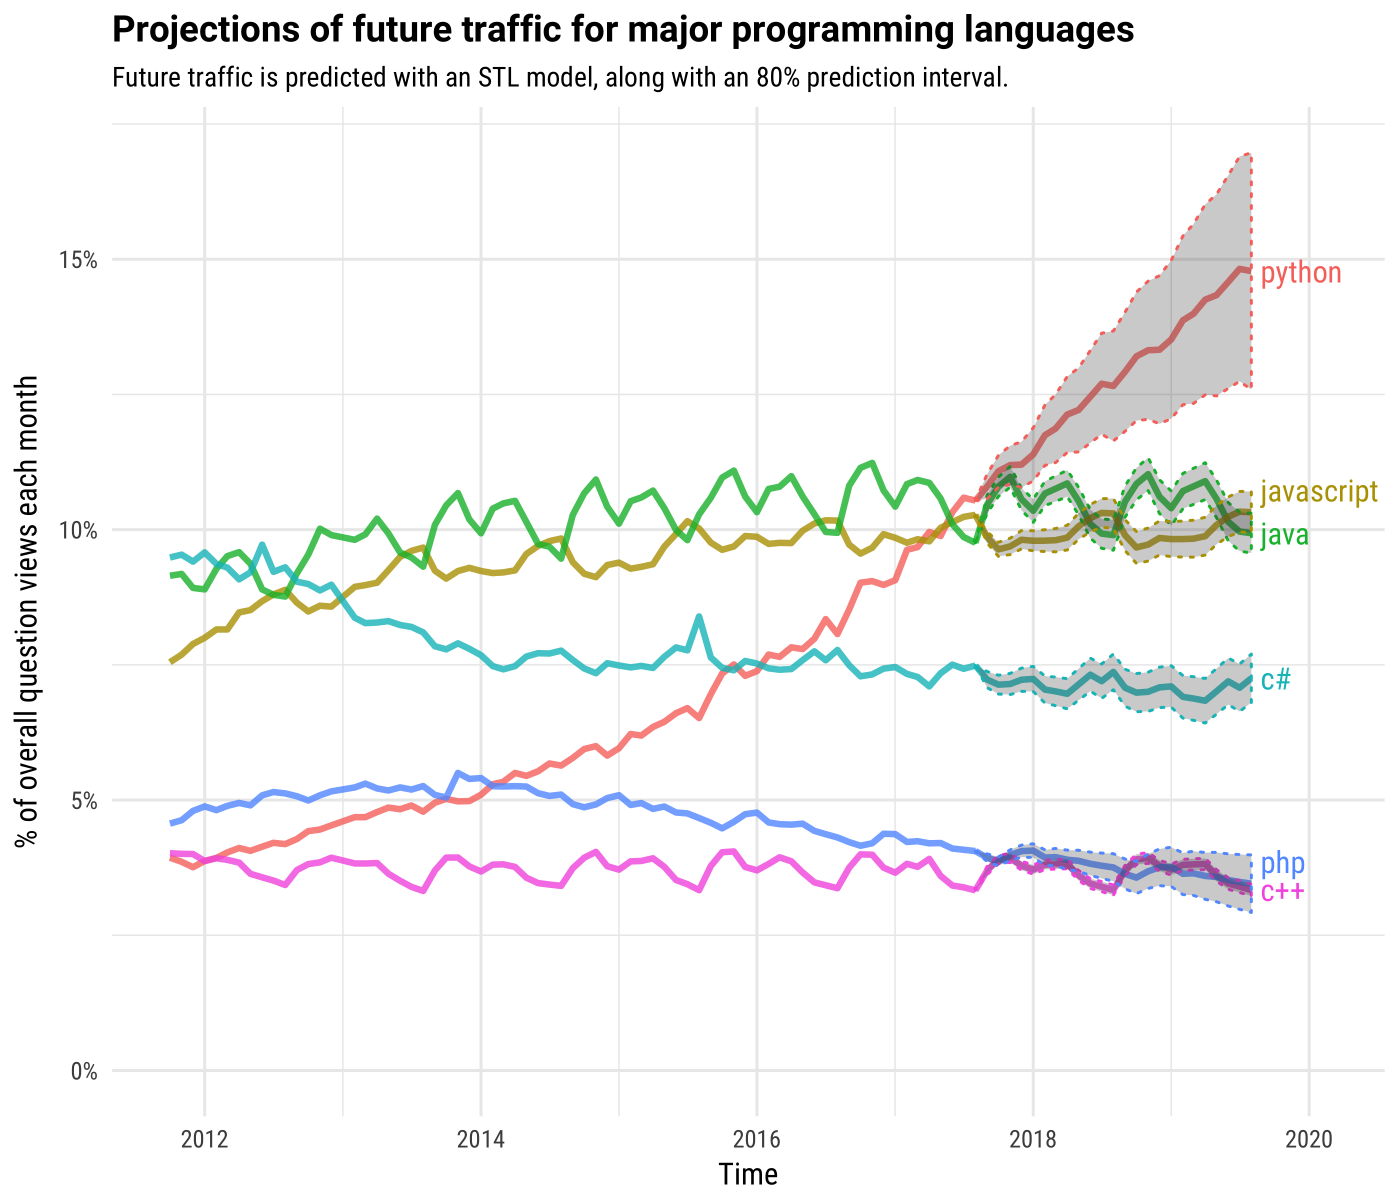
\includegraphics[width=\textwidth]{Figures/DataGeneration/projections-1-1400x1200.png}
    \caption{2018 projections of future internet traffic for major programming languages. Adapted from \cite{theoverflow}.}
    \label{fig:popularity}
\end{figure}


One of the reasons behind this tendency shift is the popularity of the language among machine learning and data science communities, fields where Python holds the first place by usage \cite{githubblog}. 
Since data-driven paradigms currently conform the state-of-the-art of many applied sciences, including audio signal processing, the availability of convenience Python packages and libraries is therefore of the highest interest to the research community. 

It is important to remark the predominant position that Matlab has always had regarding scientific computing. Indeed, it is still the tool of choice for many researchers, and the availability of libraries is accordingly very high. 
But the aforementioned tendency shift towards Python causes, as a side effect, the lack of many tools developed in Matlab by the research community.

Although Matlab code can be called and executed from Python, in practice this approach is suboptimal under several criteria. A better solution in the long run is the effective port of the code towards native Python code. Some of the libraries presented in this Chapter are partially or totally  motivated by this scenario.

	

\section{MASP: a Python library for multichannel acoustic signal processing}

\subsection{Description}

The Multichannel Acoustic Signal Processing (\textit{MASP}) is a Python library consisting of a collection of methods related with acoustics and microphone array processing.
The library is mostly a transcoding from several Matlab libraries by A. Politis\cite{politis2016microphone, github_politis}. 
It can be conveniently installed using \textit{pip}.

\textit{MASP} implements a variety of methods for the simulation and analysis of reverberant acoustic scenes, with emphasis on microphone arrays with spherical geometries.
More specifically, MASP is structured in submodules, with the following structure :

\begin{description}

	\item [Array Response Simulator] Simulation of
spherical microphones:
	\begin{itemize}
		\item Rigid/open configurations.
		\item Scattering simulation.
		\item Arbitrary capsule distances, positions and directivities.
	\end{itemize}
	
	\item [Shoebox Room Model] Fast implementation of the Image Source Method \cite{imagemethod}:
	\begin{itemize}
		\item Convex 3D rooms.
		\item Arbitrary number of sources and receivers, with arbitrary positions, orientations and directivities.
		\item ISM expansion limited by order or time.
		\item Frequency-dependent wall absorption.
		\item RIR with spherical harmonic expansion.
	\end{itemize}
	
	\item [Spherical Array Processing] Transformation and analysis of signals measured with a spherical microphone array:
	\begin{itemize}
		\item A2B conversion with theoretical or measured filters.
		\item Signal-independent beamforming.
		\item Signal-dependent and adaptive beamforming.
		\item Direction of Arrival estimation.
		\item Diffuseness estimation.
	\end{itemize}
	
	\item [Spherical Harmonic Transform] Mathematical convenience tools.
\end{description}

The library implements a Unit Testing system, which numerically assesses the validity of the methods. 
More specifically, each function test calls the equivalent Matlab code under the hood. The numeric result is then sent back to Python, where
it is evaluated against the own result.\\

Two example applications of the library are shown in Figures~\ref{fig:array_response} and \ref{fig:sht_filters}.
In Figure~\ref{fig:array_response} , obtained with the Array Response Simulator package, the frequency response of a spherical microphone array to an impinging plane-wave with varying incidence angle is shown. The microphone array consists of a 2nd order supercardioid and a 3rd order hypercardioid, located at opposite directions of an open sphere, and both of them facing to the front direction. \\

\begin{figure}[h!]
\label{fig_architecture}
  \centering
    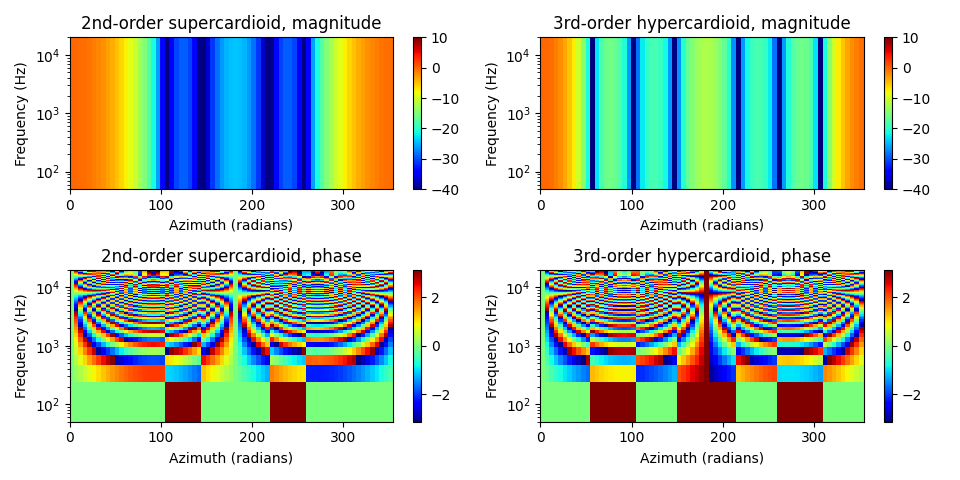
\includegraphics[width=\textwidth]{Figures/DataGeneration/array_response.png}
    \caption{Frequency response of an arbitrary spherical array.}
    \label{fig:array_response}
\end{figure}


One of the features of the Spherical Array Processing package is shown in Figure~\ref{fig:sht_filters}. The plot shows the evaluation of radial filters $\Gamma_n(kR)$ for an arbitrary spherical array, generated by inverting the theoretical response of the array \cite{Bertet2006}. 
The evaluation is performed following the metrics presented in the same paper, which compare spatial correlation, level difference and maximum amplification with respect to the ideal case. \\

\begin{figure}[h!]
\label{fig_architecture}
  \centering
    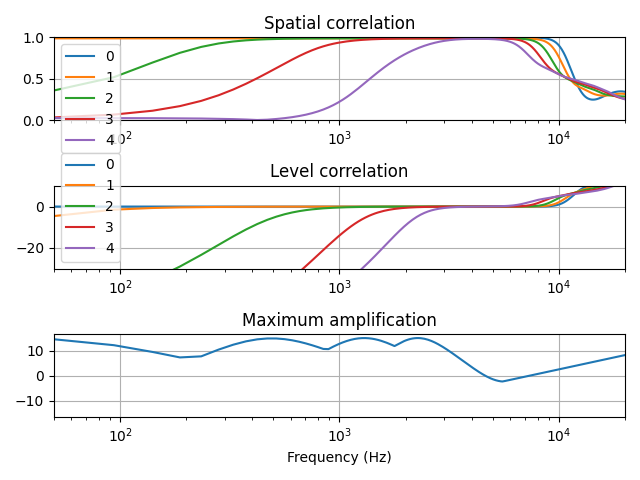
\includegraphics[width=1\textwidth]{Figures/DataGeneration/sht_filters.png}
    \caption{Evaluation of radial filters for an arbitrary spherical microphone array.}
    \label{fig:sht_filters}
\end{figure}

\subsection{Related software}

There exists another recent Python library which covers a similar scope: \textit{pyroomacoustics} \cite{scheibler2018pyroomacoustics}.
This framework provides an object-oriented interface with two main application scopes: allow RIR simulation of complex rooms based on the image source method, and provide a reference implementation of standard microphone array processing algorithms. 

Although some of the features are common to both libraries, there is a significant difference regarding their target usage. While \textit{MASP} primarily focuses on spherical geometries, \textit{pyroomacoustics} is more concerned about arbitrary room geometries and computational performance. 
Therefore, both libraries might be considered as complementary to some extent. 
A comparative list of their features is shown in Table~\ref{tab:masp_features}.



\begin{table}[th!]
\centering
\caption{Features of \textit{MASP} compared to \textit{pyroomacoustics}.}

\begin{tabular}{cccc}
  \toprule
Package & Feature &  MASP & PRA \\
\midrule
Shoebox & Convex 3D room         & \checkmark	& \checkmark \\
Room    & Non-convex 3D room     & -    			& \checkmark   \\
Model   & Arbitrary \#sources    & \checkmark   & \checkmark      \\
 & Arbitrary \#receivers, arrays & \checkmark   & \checkmark   \\
& ISM by max\_order                                 & \checkmark                              & \checkmark                              \\
& ISM by max\_time                                  & \checkmark                              & -                              \\
& Wall absorption                                   & \checkmark                              & \checkmark                              \\
& Frequency-dependent absorption                    & \checkmark                              & -                              \\
& Plot methods                                      & -                              & \checkmark                              \\
& RIR rendering                                     & \checkmark                              & \checkmark                              \\
& Audio simulation                                  & \checkmark                              & \checkmark                              \\
& Acoustic descriptor estimation                    & \checkmark                              & -                              \\
& Microphone orientation                            & \checkmark                              & -                              \\
& Custom microphone directivity                     & \checkmark                              & -                              \\
& RIR Spherical Harmonic Expansion                  & \checkmark                              & -                              \\

\midrule
Array   	& Rigid spherical arrays   & \checkmark                              & -     \\
Simulator 	& Arbitrary capsule geometries & \checkmark   & -  \\
           	& Recorded array IRs  & \checkmark                              & - \\
\midrule
Spherical & A2B conversion   & \checkmark      & -       \\
Processing  & Beamforming          		 & \checkmark      & \checkmark                              \\
 & Plane-wave decomposition         		 & \checkmark      & -                              \\
 & Nullformer                            & \checkmark      & -                              \\
& Adaptive Beamforming                   & \checkmark      & -                              \\
 & Adaptive Filtering             		 & -               & \checkmark                              \\
& DoA Estimation                         & \checkmark      & \checkmark                              \\
 & Diffuseness Estimation             	 & \checkmark      & -                              \\
 & Diffuse-field coherence               & \checkmark      & -                              \\
 & Blind Source Separation               & -               & \checkmark          \\                   
\bottomrule
 
\end{tabular}
\label{tab:masp_features}
\end{table}



\section{SOFA}

\subsection{Problem statement}

The availability of recorded room impulse responses is of great importance to many acoustic signal processing problems. 
Many different RIRs can be obtained from the same room, just by varying the position of the source and the receiver; when the number of source and receiver positions increases, the total amount of measurements increases geometrically. 
Besides that, the final format and organisation of the produced data (not only the RIR themselves, but also the source/position annotations) can be arbitrarily different when produced by different groups of people.

In order to overcome potential interoperatibility and reusability issues, the \textit{Spatially Oriented Format for Acoustics} (SOFA) convention \cite{majdak2013spatially}, also known as the \textit{AES-69} standard \cite{majdak2015aes69}, proposes a unified file format for the storage of IR-related data. 
Despite that SOFA was initially created with an emphasis on \textit{Head-Related Impulse Response} (HRIR) data, the framework that SOFA provides can be potentially applied to a variety of recording procedures and audio-related data. 
Such variety is associated with the concept of \textit{conventions}: a specific data structure designed to hold a concrete type of data or measurement. Some examples of widespread conventions might be \textit{SimpleFreeFieldHRIR} (for anechoic binaural measurements), \textit{SimpleHeadphoneIR} (intended for storing headphone impulse responses), or \textit{MultiSpeakerBRIR} (for binaural RIRs measured from loudspeaker arrays), to name a few of them.


\subsection{Ambisonics Directional Room Impulse Response as a SOFA convention}

Given the intrinsic spatial characterization capabilities of ambisonics, Gerzon proposed the technique as a potentially successful candidate format for acoustical heritage preservation, as early as 1975 \cite{gerzon1975recording}.

The increase in popularity of ambisonics since the beginning of the present century has turned this idea into reality; OpenAIRlib, a freely accesible dataset that gathers dozens of RIRs, might be a good example of it \cite{openair}.

In any case, the usage of recorded ambisonic RIRs is not limited to the field of acoustic heritage. Among others, the availability of such recordings has powered works in a variety of works, auralization \cite{postma2016virtual}, room acoustics analysis \cite{embrechts2015measurement,clapp2011investigations} and modelling \cite{romblom2017diffuse}, spatial audio synthesis \cite{coleman2017object} or source separation \cite{baque2016separation}. \\


In general, all publicly available ambisonic RIR measurements share some common approaches for describing and organizing the recorded data. 
For instance, recordings from different rooms are usually stored as separated folders. 
Each combination of emitter and receiver positions is often saved as an individual file, and the different spherical harmonics match the audio channels.
Moreover, it is also usual to provide a \textit{metadata} file, describing the different emitter and receiver positions, and potentially some information about the measurement setup, methodology, etc. Such files might be formatted as plain text or delimiter-separated files.
 
Despite the common approach, it can be easily foreseen that each database generated by a different individual or institution might potentially have a different naming convention, folder structure, file format, and so on. 
This is exactly the same situation that motivated the development of the SOFA conventions. 

On the other hand, the SOFA specification defines some criteria that must be fulfilled in order to propose a new convention \cite{sofaconventions}. These criteria are:
\begin{enumerate}
    \item Data must exist.
    \item Data can not be described by existing SOFA conventions.
    \item Relevant information about the data must be available.
\end{enumerate} 

Given that the described situation meets all requirements, the \textit{Ambisonics Directional Room Impulse Response} (AmbisonicsDRIR) convention has been therefore proposed as a new member of SOFA.\\

The technical specifications of the proposed convention in its current state (version 0.2) are available online \cite{ambisonicsdrir}. 
Despite a timid adoption of the convention, the AmbisonicsDRIR proposal has arisen interest in the community. At the moment of writing, the \textit{Standardisation Committee on AES-69 Standard} is discussing potential modifications to the SOFA file format required for the adoption of several new features; and the support for spherical harmonic-based measurements is among the topics for deliberation.


\subsection{pysofaconventions}

The situation described in Section~\label{sec:intro_data}, regarding the availability of acoustic signal processing libraries in the Python programming language, can be easily extended to the case of SOFA APIs.
 
The library \textit{pysofaconventions} has been created with the aim to provide an alternative to the existing Matlab/Octave and C/C++ implementations. 
For ease of installation, it is integrated in the standard python package manager, \textit{pip}. 

The current software version is 0.1.5. The library structure is inspired by the C++ implementation \cite{api_cpp}. 
It features all functionalities described by SOFA version 1.0, plus the proposed AmbisonicsDRIR convention. 
The implementation is based on extensive error checking, to ensure code consistency.
 
\textit{pysofaconventions} has gained a moderate amount of attraction. Among others, it is being used as a dependency for the \textit{Real-Time Spherical Microphone Renderer (ReTiSAR) for binaural reproduction}, developed by Chalmers University in collaboration with Facebook Reality Labs \cite{helmholz2019real}.


\section{Ambiscaper}


%
%Explain about mono files plus ambisonics IRs.
%
%
%\section{Recorded IRs}
%
%
%Impulse Responses (IRs) measurements constitute a compact way of representing the acoustic propertiesof a linear time-invariant system. When such measurements are performed in a specific room or enclosure, the so-called Room Impulse Responses (RIRs) are able to capture the intrinsic reverberation and acoustic characteristics of the enclosure, for which several methods have been developed these past years \cite{stan2002comparison}. Furthermore, it is possible to account for different emitter/receiver positions in the measurement, usually performing the measurement with a microphone array. In that case, this kind of measurements is referred to as Directional Room Impulse Responses (DRIRs) \cite{embrechts2005computation}. DRIRs have a wide range of applications: auralization \cite{embrechts2005computation}, room acoustics analysis \cite{embrechts2015measurement,clapp2011investigations} and modelling \cite{romblom2017diffuse}, spatial audio synthesis \cite{coleman2017object}, source separation and dereverberation \cite{baque2016separation}, acoustic heritage preservation \cite{gerzon1975recording,murphy2005multi}, etc. 
%
%
%\subsection{Ambisonics Recording}
%
%It is also possible to capture Ambisonics audio scenes by using specific recording devices. Spherical microphone arrays (also known as \textit{Ambisonics microphones}) are a type of microphone arrays in which the capsules are located around a spherical surface, presenting rotational symmetry. Such geometric arrangement allows the recorded signals to be transformed to the Ambisonics domain, by means of projection into the Spherical Harmonics basis, and further equalization with radial filters \cite{Bertet2006}.
%
%This process is known in the audio production domain as \textit{A-B Conversion}. All major spherical microphone array manufacturers provide tools for achieving this transformation \cite{soundfield,ambeo,zylia,tetra,em32}.
%
%
%\subsection{Ambisonics DRIRs}
%
%The intrinsic spatial capabilities of Ambisonics microphones might be applied to DRIR recording, as originally proposed by Gerzon in the context of acoustical heritage preservation \cite{gerzon1975recording}. In recent years, several datasets of Ambisonics DRIRs have been publicly released, such as the OpenAIR database \cite{murphy2010openair} or the set of  measurements performed in the scope of the S3A project \cite{coleman2015s3a,openair}. 
%
%\subsection{The SOFA Conventions}
%
%In general, the Ambisonics DRIR databases show a common approach for describing the measurements: given a specific room, usually represented as a folder, IR data consist of several multichannel audio files, with one audio channel per spherical harmonic, and one file per emitter/receiver combination. Furthermore, it is also usual to provide a \textit{metadata} file, describing the different emitter and receiver positions, and eventually some information about the measurement setup, methodology, etc. Such files might be formatted as plain text or delimiter-separated value files.
%
%Despite the common approach, it can be foreseen that each database generated by a different individual or institution might potentially have a different naming convention, folder structure, file format, and so on. This situation hinders data manipulation and exchange, and forces users to write ad-hoc parsers and algorithms for each specific database.
%
%The \textit{Spatially Oriented Format for Acoustics} (SOFA) is a file format designed for a consistent, standardized storage and manipulation of IR data \cite{majdak2015aes69}. The need for such standard arose from dealing with different databases of \textit{Head-Related Transfer Functions} (HRTFs), in a similar manner as the one mentioned for Ambisonics DRIRs.
%
%There are several SOFA conventions, each one addressing a particular type of IR measurement. In the case of Ambisonics DRIRs, given the data representation in existing databases, one could outline the following specificities:
% 
%\begin{itemize}
%    \item Presence of Ambisonics-related information (Ambisonics order, channel ordering and normalization)
%    \item Audio stored in the Ambisonics (spherical harmonics) domain  
%    \item Data structure support for different combinations of source and receiver positions
%\end{itemize}
%
%
%However, none of the existing SOFA conventions meets those requisites. The potentially first candidate by name, \textit{SingleRoomDRIR}, is limited to one source position per file. On the other hand, \textit{MultiSpeakerBRIR} allows for multiple sound sources, but restricts the number of receivers (microphone capsules) to two, as expected in a binaural recording. \textit{GeneralFIRE} is intended for "data which are too general to store in more specific conventions" \cite{generalfire}.
%
%
%\subsection{Convention Proposal}
%
%\subsubsection{Considerations}
%
%The SOFA specification defines some criteria that must be fulfilled in order to propose a new convention \cite{sofaconventions}. These criteria are:
%\begin{enumerate}
%    \item Data must exist.
%    \item Data can not be described by existing SOFA conventions.
%    \item Relevant information about the data must be available.
%\end{enumerate}
%
%
%As we already mentioned, existing databases of Ambisonics DRIRs can be found in OpenAIR and S3A databases (criterium 1). Criterium 2 has been discussed in the previous paragraph. All available Ambisonics DRIR datasets are accompanied by explanations, pictures, diagrams and related information (criterium 3). 
%
%\subsubsection{Specifications}
%
%We therefore propose a new SOFA convention, \textit{AmbisonicsDRIR}, designed for DRIRs measured with spherical microphone arrays, and presented in the Ambisonics domain. In other words, we propose to store the instantaneous $B_{mn}$ values for a given Ambisonics order $L$, provided that $S$ is a unit impulse (Eq. \ref{eq1}).
%
%The \textit{Listener} - as defined by the SOFA specification - is embodied by the spherical microphone array. The different \textit{Receivers} are the different Ambisonics Components $B_{mn}$, so that their number is fixed provided $L$ (more precisely, by following the relationship $R = (L+1)^2$), and their positions are not applicable. Furthermore, there might be many different \textit{Sources}, all of them omnidirectional and consisting of one only \textit{Emitter}. In that sense, \textit{M} represents the number of different \textit{Source} positions. 
%
%
%The proposed convention is based on \textit{GeneralFIRE}, with the following modifications:
%\begin{itemize}
%
%    \item Mandatory field \textit{GLOBAL:AmbisonicsOrder} (type \textit{double}, dimension \textit{I}, default \textit{1}). Indicates the order of the Spherical Harmonic expansion.
%    
%    \item Mandatory field \textit{DATA:ChannelOrdering} (type \textit{attribute}, default \textit{acn}). Describes the ordering of the different Ambisonics Channels. Must be one of: \textit{acn} or \textit{fuma}.
%    
%    \item Mandatory field \textit{DATAChannelNormalization} (type \textit{attribute}, default \textit{sn3d}). Describes the Ambisonics normalization convention used in the data. Must be one of: \textit{sn3d}, \textit{n3d}, \textit{fuma} or \textit{maxn}.
%    
%    \item Fields \textit{ReceiverPosition}, \textit{ReceiverPosition:Type} and \textit{ReceiverPosition:Units} are not needed, since it is assumed that \textit{Receivers} represent the Ambisonics channels. Furthermore, the values of \textit{R} (number of receivers) are defined by $R = (L+1)^2$. Accordingly, the values of \textit{GLOBAL:AmbisonicsOrder} and \textit{R} are valid only if they follow the given equation.
%    
%    \item Field \textit{DATA:Delay} is not mandatory.
%    
%    \item Relevant information about the microphone model and brand, Ambisonics encoding methodology, software used, etc, is recommended to be added into the field \textit{GLOBAL:Comment}.
%    
%\end{itemize}
%
%\subsection{Results}  
%
%As a preliminary result, we have extended the current SOFA C++  \cite{sofacpp} and Matlab \cite{sofamo} APIs to be fully compatible with the AmbisonicsDRIR convention. \todo{pysofaconventions}
%
%Furthermore, as a use-case, a selection of existing Ambisonics DRIRs have been transcoded to the proposed convention: \textit{Emmanuel Main Church} from S3A database \cite{coleman2015s3a}, and \textit{Heslington Church} and \textit{York Guildhall Council Chamber} from the OpenAIRlib \cite{openair}. Figure \ref{guildhall} shows a schematic diagram of the different \textit{Emitter/Receiver} positions at the \textit{York Guildhall Council Chamber} recordings. The data, as well as the tools used to perform the conversion, are available online under an open source license \cite{ambisonicsdrirexamples}.
%
%Finally, we must remark that the \textit{AmbisonicsDRIR} SOFA convention proposal is currently under discussion, and the described specifications are subject to change with upcoming versions. 
%
%% TODO: include some examples!!! about data dimensions etc
%
%\begin{figure}
%	\centering
%	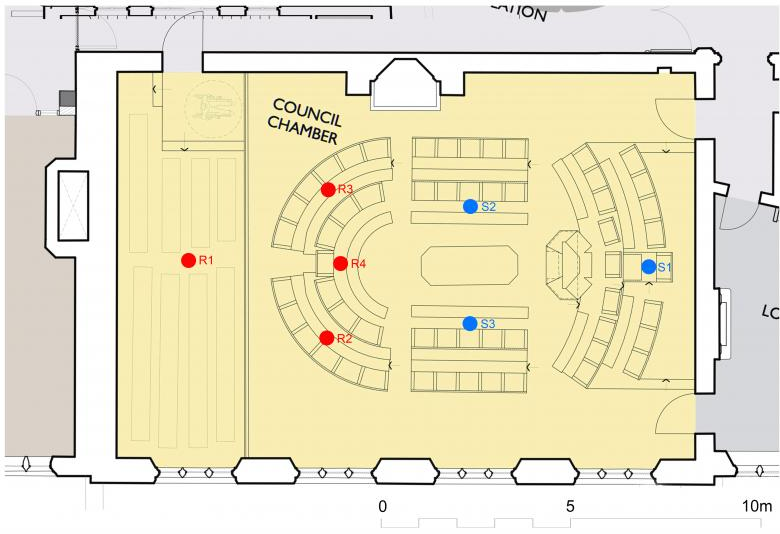
\includegraphics[width=\textwidth]{Figures/DataGeneration/guildhall}
%	\caption{Source and Listener position diagram for the "York Guildhall Council Chamber" Ambisonics DRIR (original diagram attribution to \cite{guildhall} }
%	\label{guildhall}
%\end{figure}
%
%\subsection{Summary} 
%
%This document addresses the lack of compatibility among different databases of Ambisonics DRIRs. The present proposal consists in defining a new SOFA convention, specifically designed for Ambisonics DRIRs. That way we contribute to improve the ease of data manipulation and database interoperability. Software implementations and tools for automatic conversion are provided.
%
%
%
%\section{Simulated IRs}
%
%explain different methods and libraries.
%tell about masp.
%
%
%
%
%
%
%% ==================================================================
%\section{High-level scene description}
%
%\subsection{Motivation}
%
%\todo{introduce the topic}
%
%\todo{ARRANGE this introduction in a meaningful way}\\
%The work by Moore \cite{Moore2015} was the first to combine Intensity Vector statistics with DPD-test preprocessing. A similar approach is found on the \textit{Single Source Zones (SSZs)} algorithm, first presented by Pavlidi \cite{Pavlidi2015}. Other recent proposals, as for example the work by He \cite{He2017}, consider the local DOA variance as an estimator of reliability. 
%
%Source Localization based on IV statistics has been also successfully used as a preprocessing step for Source Separation tasks. The proposal of G\"unel \cite{Gunel2008}, which uses beamforming over the DOA estimation, was a pioneer work on this scope. Other similar approaches, which rely on DOA-based Time-Frequency (TF) masking, can be found on the works by Shujau \cite{Shujau2011}, Riaz \cite{Riaz2015} or Chen \cite{Chen2015}.
%
%
%
%\subsection{Evaluation data}
%\label{subsec:evaluationdata}
%
%Audio data used for evaluation in the works presented in Section \ref{subsec:algorithms} can be classified in  three main categories:
%
%
%\begin{itemize}
%
%    \item \textit{IR simulations:} Impulse Responses simulated by numerical methods, using software tools such as \textit{SMIR Generator} \cite{smir}. IR simulation provides the most flexible approach for evaluation, since it allows custom design and parametric analysis (algorithm evaluation as a function of reverberation time, source(s) distance(s), etc). However, the resulting audio data realism is restricted by the simulation algorithm, which is usually limited to empty \textit{shoebox} rooms.
%    
%    \item \textit{IR recordings:} Impulse Responses (IRs) of specific rooms recorded with an Ambisonics microphone, as first presented by Gerzon in the context of acoustic heritage preservation \cite{gerzon1975recording}. IR recordings do not provide the flexibility of IR simulations, but allow realistic captures of the room's acoustic properties, while maintaining the potential of using different source contents and positions. OpenAIRlib \cite{murphy2010openair} is the reference public repository for IRs, even including a dedicated Ambisonics IR section.
%
%    \item \textit{Audio recordings:} a sound scene recorded in a specific room, using an Ambisonics microphone and real sound sources. This approach  represents the  most  accurate  option  for algorithm evaluation in a real scenario. However, its cost and lack of flexibility makes this approach only attractive for last stages of algorithm  evaluation.
%
%\end{itemize}
%
%In the case of IR simulations and recordings, the Ambisonics IRs are convolved with anechoic monophonic recordings to produce the actual evaluation data. The anechoic recordings are usually taken from standard audio processing databases, such as TIMIT \cite{timit}. \\
%
%Table \ref{table:evaluationdata} summarizes the evaluation data types used in each work review in Section \ref{subsec:algorithms}, along with the audio content type and origin database (if any).    
%
%
%%% DOA ESTIMATION
%\begin{table}[htpb]
%    \centering
%    \footnotesize
%
%	\begin{tabular}{ p{2cm} p{2.8cm} p{2.5cm} p{2.3cm} }
%    \toprule
%    % \cmidrule(r){1-2}
%    
%    % \centering 
%    \textbf{Article} &
%    % \textbf{\textit{$L$}} &
%    \textbf{Evaluation Data Type} &
%    \textbf{Audio Content Type} &
%    \textbf{Database}\\
%    \midrule
%    
%    Thiergart \cite{thiergart_localization_2009}
%    % & 1 h
%    & Audio recording 
%    & Speech
%    & -\\
%    
%    Tervo \cite{Tervo2009}
%    % & 1 h
%    & Audio recording
%    & Noise, music
%    & -\\
%    
%    Jarret \cite{Jarrett2010} 
%    % & 4 
%    & IR simulation, Audio recording
%    & Noise
%    & -\\
%    
%    Nadiri \cite{Nadiri2014}   
%    % & 4 
%    & IR simulation, Audio recording
%    & Speech
%    & TIMIT \\
%    
%    Moore \cite{Moore2015}   
%    % & 4 
%    & IR simulation 
%    & Speech
%    & APLAWD \\
%    
%    Pavlidi \cite{Pavlidi2015}
%    % & 4
%    & IR simulation 
%    & Noise, speech
%    & -\\
%    
%    He \cite{He2017}   
%    % & 1 h
%    & IR simulation, Audio recording
%    & Speech
%    & TIMIT \\
%
%    
%    % Ding \cite{Ding2017}   
%    % % & 1 h
%    % & IR simulation \& Audio recording \\
%    
%    \midrule
%    
%    Gunel \cite{Gunel2008}
%    & IR recording
%    & Speech, music
%    & Music for Archimedes \\
%    
%    Shujau \cite{Shujau2011} 
%    & Audio recording
%    & Speech
%    & TIMIT \\
%    
%    Riaz \cite{Riaz2015}
%    & IR recording
%    & Speech, music
%    & Music for Archimedes \\
%    
%    Chen \cite{Chen2015}
%    & IR simulation, IR recording
%    & Speech
%    & TIMIT \\
%
%    \bottomrule
%    \end{tabular}
%    \caption{Summary of audio data used across Ambisonics-based Source Localization (above) and Source Separation (below)  algorithm proposals. \todo{update table? fix references}}
%    \label{table:evaluationdata}
%\end{table}
%
%
%
%Although algorithm evaluation in real scenarios provides the most realistic approach to the problem, this methodology has not been widely adopted due to its cost and lack of flexibility. As an example, none of the works using real recordings in Table \ref{table:evaluationdata} performs the evaluation with more than one  recording in each case. In contrast, when using IR-based  scenes, the number of audios evaluated are usually one or two magnitude orders greater. 
%
%However, it is important to notice the lack of public availability of evaluation data. None of the analyzed articles provide a way to access neither the used audio dataset, nor the groundtruth (position annotations in the case of Sound Localization, and original sound sources for Sound Separation). Only in the case of simulated IRs it is possible to partially replicate the experimental setup, since some of the parameters used in the simulation software are usually provided. Furthermore, the process of creation of the custom datasets (selecting an anechoic audio dataset, convolving with custom IRs, or performing real recordings) seems to be performed \textit{ad-hoc} on each article. 
%
%Taking into account the flexibility offered by IR-based scenes, it would be desirable to have a tool for automatic generation of reverberant Ambisonics scenes (and their associated groundtruth) for analysis purposes. Such tool would help the scientific community in several ways: reducing the amount of time dedicated to build custom datasets, reusing publicly available resources and recordings, and enhancing experiment reproducibility by making easier the exchange of datasets. Furthermore, the capacity of producing a big number of diverse audio scenes for analysis will help the algorithm design and early testing stages,and specially the training stage of machine learning-based algorithms. 
%
%
%\subsection{AMBISCAPER}
%\label{sec:ambiscaper}
%
%\todo{this has been downgraded to subsection. maybe place it at the introduction or something to find a more meaningful explanation}
%
%AmbiScaper \cite{ambiscaper} is a tool designed to provide a flexible way of creating complex Ambisonics sound scenes and their associated groundtruth, to be used in the context of Source Localization and Source Separation algorithms.
%AmbiScaper offers a high level control of the sound scene parameters, and provides an easy way of creating large datasets with custom characteristics.
%AmbiScaper is based on Scaper, a framework designed to generate ground truth information to train Sound Event Detection models \cite{Salamon2017}.
%
%\subsection{Sound scene description}
%\label{subsec:description}
%
%One of the main features of AmbiScaper is that all parameters of the sound scene can be specified in a non-deterministic way. In that sense, the parameters for each \textit{event} (sound source) are actually generated through a two-step process. First, in the \textit{Event Specification}, all parameters related to an event are defined in terms of statistical distributions. During the \textit{Event Instanciation}, the actual values for each parameter are then sampled from the statistical distributions.
%This two-step process allows the user to describe abstract \textit{templates} of sound scenes, rather than manually assigning values to parameters. Therefore, a single \textit{event specification} might produce potentially infinite different sound scenes. 
%
%
%
%\subsection{Architecture}
%\label{subsec:architecture}
%
%\begin{figure}
%\label{fig_architecture}
%  \centering
%    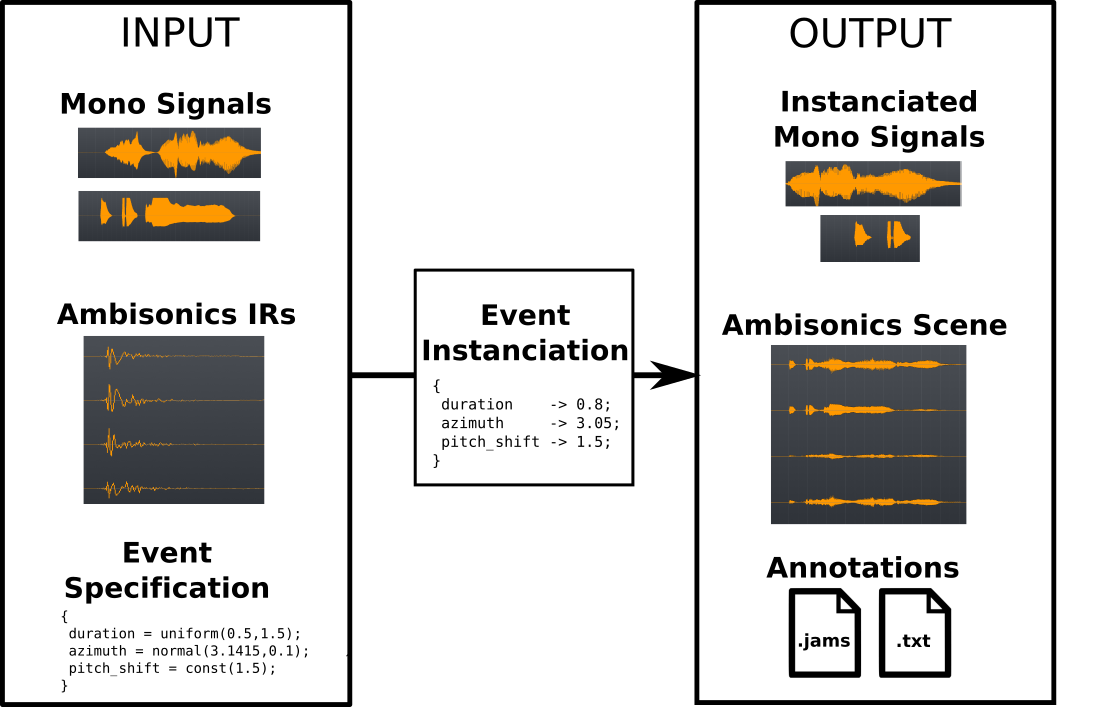
\includegraphics[width=\textwidth]{Figures/DataGeneration/figure_architecture_V2.png}
%    \caption{AmbiScaper architecture.}
%\end{figure}
%
%%%%%%%%%
%In order to generate a sound scene, AmbiScaper requires three different inputs: the original \textit{mono signals}, which will be the basis for the scene's audio content, an optional \textit{Ambisonics IR}, and the \textit{event specification}. 
%
%The process of dataset creation starts with the \textit{event instanciation}, as described in Section \ref{subsec:description}. Once all values are sampled, three different types of output are generated: the \textit{Ambisonics scene}, the \textit{instanciated mono signals} (the original mono signals after data augmentation and duration changes), and the \textit{annotations}, in the form of a JAMS file \cite{humphrey2014jams}, containing all information about the scene specification and the instanciated values. 
%
%AmbiScaper's architecture is depicted in Figure \ref{fig_architecture}.
%
%
%\subsection{Reverberation}
%
%When no reverberation is specified, AmbiScaper can generate anechoic sound scenes, which can be useful for baseline performance evaluation. In this case, there is no upper limit on the Ambisonics order of the rendered scene. Furthermore, the anoechic case allows for the specification of source \textit{spread} or apparent size through Ambisonics order downgrade \cite{carpentier2017ambisonic}.
%
%AmbiScaper supports the usage of recorded Ambisonics IRs, although it is currently limited to IRs from the S3A database \cite{coleman2015s3a}. The development of a standardized file format for Ambisonics IRs, which is being discussed at the moment of writing, will provide the flexibility to work with arbitrary Ambisonics IRs.   
%
%Lastly, AmbiScaper features the possibility of using simulated Ambisonics IRs, through a wrapper to \textit{SMIR Generator}. In this case, the reverberation model specifications might be defined as well in statistical terms, and the generated IRs are stored for evaluation purposes. A working copy of Matlab is required to run this option.
%
%When a reverberant sound scene is created, the specific Ambisonics IRs used on the scene are also provided as an output. Other research problems such as dereverberation or room reflection modelling might therefore benefit from such data.
%
%
%
%
%\subsection{AmbiScaper and experiment reproducibility}
%
%As mentioned in Section \ref{subsec:evaluationdata}, there is a generalized lack of publicly available datasets for Source Localization and Source Separation in the Ambisonics domain. Even when using general purpose audio/speech datasets (such as TIMIT), the actual reverberant Ambisonics evaluation data is usually not available.
%In that sense, the compatibility of AmbiScaper with public Ambisonics IR databases is a key aspect for reproducibility, since it allows for the reutilization of acoustical measurements in a systematic way.
%
%Furthermore, the output of the AmbiScaper dataset generation process is not limited to the actual dataset. In fact, as explained in Section \ref{subsec:architecture}, the resulting annotation file does not only contain the \textit{instanciation} (the actual values of each parameter in the sound scene), but also the \textit{specification} (the statistical distributions from which the instanciated values are sampled). In the scope of experiment reproducibility, the exchange of \textit{specification files} instead of actual audio files greatly reduces the storage capacitiy and bandwith required to transfer big databases. 
%
%AmbiScaper is implemented in the form of a Python package, publicly available through the \textit{Python Package Index} repository. 
%AmbiScaper is free software under the GPL license, easing the software adoption and the potential engagement of the scientific community with the development. 
%
%
%\subsection{Sample Dataset}
%\label{ssec:dataset}
%
%As an example of the potential capabilities of AmbiScaper,  we have created and published a dataset for the evaluation of source localization algorithms \footnote{https://zenodo.org/record/1186907 \todo{link}}.
%
%The dataset contains 300 first order Ambisonics sound scenes, each one containing from one to three static sound sources (be they simultaneous or not), with different gains and SNRs, and placed at random positions around the sphere. Each sound scene has a duration between 1 and 2 seconds.
%
%The sources are randomly chosen from a subset of the Anechoic OpenAirlib database, which mostly contains recordings from baroque musical instruments.
%The AudioBooth IR database from S3A has been used for all scenes.
%It features SoundField recordings from an acoustically treated room with a geodesic dome structure, to which 17 speakers have been attached.
%
%
%
%\subsection{CONCLUSIONS AND FUTURE WORK}
%\label{sec:conclusions}
%
%AmbiScaper is a tool designed for easy dataset creation and exchange, in the context of reverberant Ambisonics Source Localization and Source Separation. It responds to the lack of public datasets for algorithm design, evaluation and reproducibility. An example dataset generated with AmbiScaper, and its analysis with state-of-the-art Source Localization algorithms are also provided.
%Further studies in Ambisonics IR position interpolation would allow creating non-static audio scenes, which might be an interesting feature. 
%Another feature in progress is the support for a standardized Ambisonics IR format \cite{perez2018ambisonics}, which will ease data reusability and provide the potential to cover a big variety of acoustic scenarios. 
%
%
%
%
%
%
%
